\documentclass[10pt,a4paper]{article}
\usepackage[left=4cm,right=4cm,top=3.5cm,bottom=1.5cm]{geometry}
\usepackage[utf8]{inputenc}
\usepackage[english]{babel}
\usepackage[T1]{fontenc}
\usepackage{amsmath}
\usepackage{amsfonts}
\usepackage{amssymb}
\usepackage{graphicx}
\usepackage{lmodern}
\usepackage{siunitx}
\usepackage{fancyhdr}
\usepackage{enumerate}
\usepackage{mathtools}
\usepackage{float}
\usepackage{csquotes}
\usepackage{multicol}
\usepackage{lipsum}
\usepackage{tcolorbox}
\usepackage{enumitem}
\usepackage{varwidth}
\usepackage{todonotes}

% Setup SI units
\sisetup{locale=DE}
\sisetup{per-mode = symbol-or-fraction}
\sisetup{separate-uncertainty=true}
\DeclareSIUnit\year{a}
\DeclareSIUnit\clight{c}
 
 % Einbinden von Bildern
\usepackage{float}
\usepackage{graphicx, subfigure}	
	\graphicspath{{img/}}
\usepackage[skip=2pt]{caption}
 
% Abkürzungen
\usepackage{glossaries}
\newacronym{mpc}{MPC}{Model Predictive Control}
\newacronym{sos}{SOS}{Sum of Squares}
\newacronym{ocp}{OCP}{Optimal Control Problem}


 
% Being of document
%----------------------------------------------------------------------

% Defintions for the Document
\begin{document}
\pagestyle{fancy}
\lhead{University of Stuttgart}
\rhead{Institute of Flight Mechanics and Control}

% parskip
\setlength{\parindent}{0pt}

%----------------------------------------------------------------------

\begin{center}
	\LARGE{\textbf{Systems Theory Project Report}}\\[0.25em]
	\normalsize\textbf{Nonlinear Model Predictive Control Design}\\[0.25em]
	\normalsize{Elias Niepötter (3684096)}
\end{center}

\vskip 0.5cm

\begin{abstract}
	% \lipsum[1]
\end{abstract}

\vskip 0.5cm

% \begin{multicols}{2}

\section{Introduction}
The goal of the project is to combine the methods of \gls{sos} Programming and nonlinear \gls{mpc}.
Based on an exemplary nonlinear dynamical system an \gls{mpc} is designed in such a way that it acts outside a specified
region in the state space and drives it towards this region. The region is called \textit{terminal region}. Inside the
terminal region a linear controller takes over, this concept is called \textit{Dual Mode Control}. \gls{sos} methods are 
used to estimate the terminal region which is a \textit{region of attraction} of the closed loop dynamics of the linearly 
controlled system.
The report first introduces the basics of \gls{mpc} in \ref{sec:mpc}. Continuing with the concept of dual mode controller 
design focussing on \gls{sos} methods in \ref{sec:synTermCond}. Lastly, the methods presented are applied to the 
ball beam system. The results are shown and discussed in \ref{sec:example}. \todo{reformulate Introduction}

\section{Model Predictive Control}
\label{sec:mpc}
Model Predicitve Control is a flexible and powerful control strategy. It naturally handles nonlinearities constraints as
well as multiple inputs and outputs. The underlying idea is based on optimal control theory. \gls{mpc} is characterized by
two key features. First, an iterative online optimization is performed to compute the next control input. Second, at each 
instance of time an \gls{ocp} is solved, therefore the time horizon of the \gls{ocp} moves forward. \cite{nmpcBible}

\begin{figure}[h]
	\begin{center}
		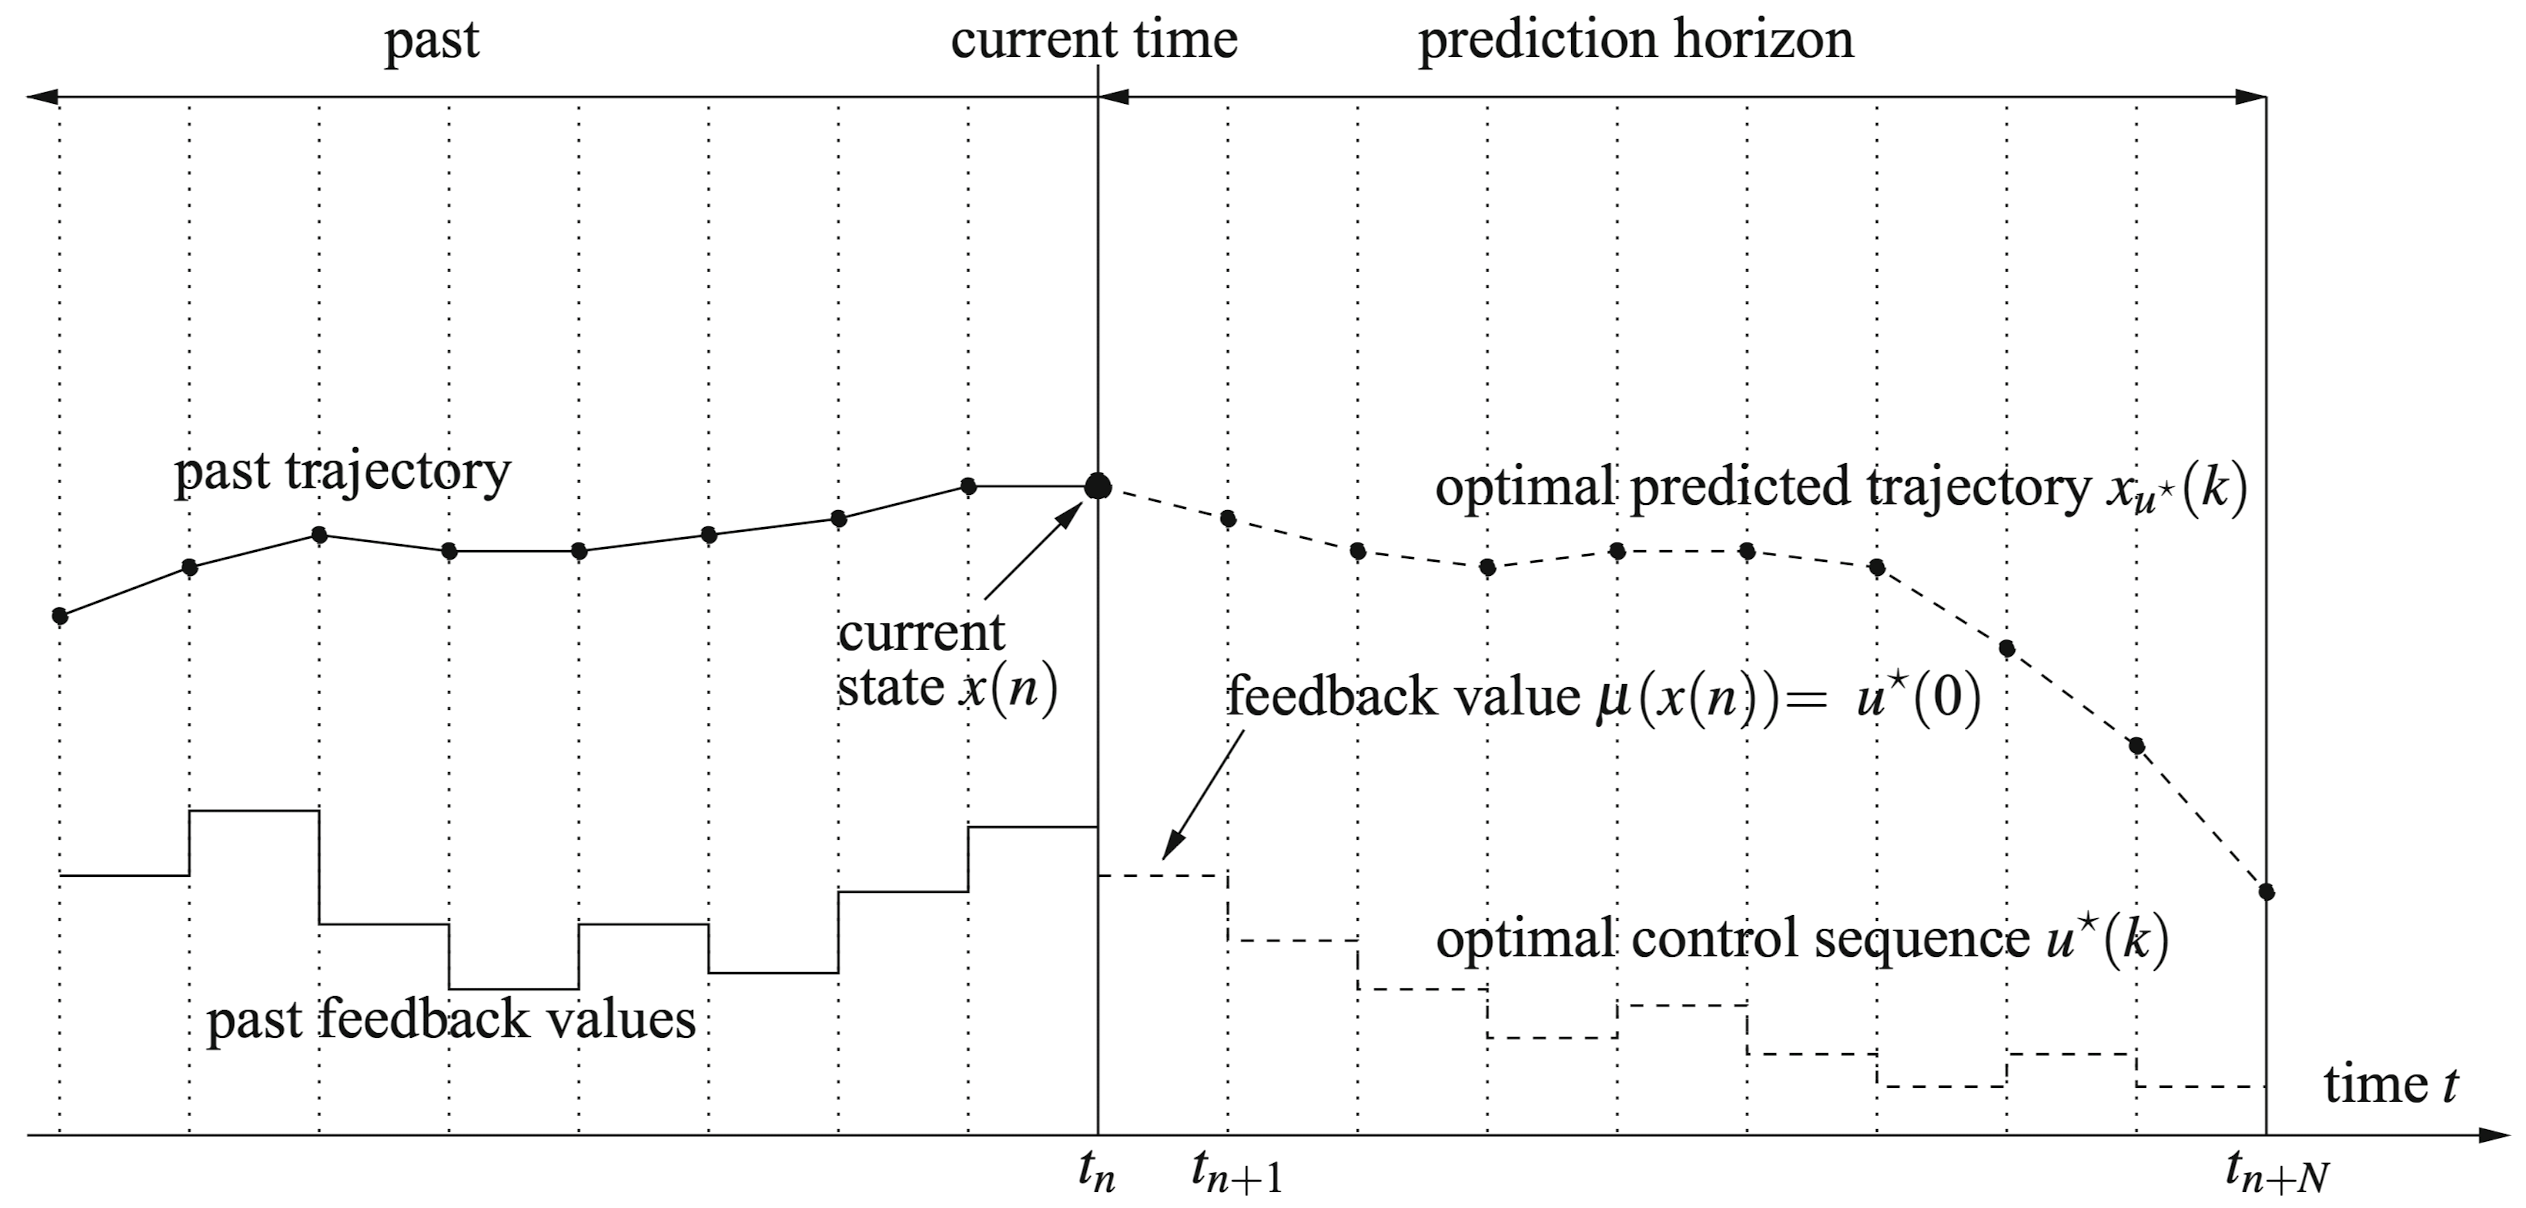
\includegraphics[width=0.8\textwidth]{img/nmpc_idea.png}
		\caption{Moving horizon and optimization of an MPC in discrete time \cite{nmpcBible}}
		\label{pic:nmpc_idea}
	\end{center}
\end{figure}

Figure \ref{pic:nmpc_idea} illustrates the two key feastures of \gls{mpc} in discrete time. At time instance $t_n$ 
the \gls{ocp} for the next $N$ time steps is solved. Given that the \gls{ocp} is feasible, the first optimal control
input $u^*_0$ is applied to the system. The system evolves to the next time instance $t_{n+1}$ and the process repeats.

\subsection{Problem Formulation}
The discrete time finite horizon optimal control problem can be formulated as follows:

\begin{align}
\label{eq:mpc_problem}
    \begin{array}{ll}
        \min\limits_{\nu} & E\left(x_{k+N \mid k}\right)+\sum_{i=k}^{k+N-1} F\left(x_{i \mid k}, u_{i \mid k}\right) \\[2em]
        \text { s.t. } & x_{i+1 \mid k}=f\left(x_{i \mid k}, u_{i \mid k}\right), \quad x_{k \mid k}=x_k\\
        & u_{i \mid k} \in \mathcal{U}, \quad i \in[k, k+N-1]\\
        & x_{i \mid k} \in \mathcal{X}, \quad i \in[k, k+N-1]\\
        & x_{k+N \mid k} \in \mathcal{E}
    \end{array}
\end{align}

where

\begin{equation}
\label{eq:mpc_costFunction}
    J\left(\nu, x_k\right)=\underbrace{E\left(x_{k+N \mid k}\right)}_{\text{terminal costs}} + \underbrace{\sum_{i=k}^{k+N-1} F\left(x_{i \mid k}, u_{i \mid k}\right)}_{\text{stage costs}}
\end{equation}

with $\mathcal{U}$ input constraints,  $\mathcal{X}$ state constraints and $\mathcal{E}$ terminal region/set as the constraining sets.
The \gls{ocp} is solved for the prediction horizon $N$, the initial condition $x_k$ at the current time step $t_k$, the dynamics
of the system given by $f\left(x_{i \mid k}, u_{i \mid k}\right)$ and the terminal state $x_{k+N \mid k}$. The cost function \eqref{eq:mpc_costFunction}
consists of the terminal costs at last time instance $t_N$ of the optimization and the stage costs for all other time instances starting from
the initial condition. The optimal control sequence is defined as

\begin{equation}
	\nu^* = [u_{k \mid k}^*, \dots , u_{k+N-1\mid k}^*]^T.
\end{equation}

The control input $\mu$ at each discrete time step $t_k$ is the first element of the optimal control sequence $\nu^*$

\begin{equation}
\mu(x(t_k)) \coloneqq \nu^*(0)
\end{equation}

See \cite{nmpcBible} and \cite{RaffAllgoewer} for details on the formulation of the \gls{ocp} resp. the \gls{mpc} formulation.

\subsection{Terminal Conditions for MPCs}
The shown \gls{mpc} includes terminal conditions. These conditions are part of the design of the \gls{mpc} and are used to
guarantee certain stability properties of the closed loop system. The followong Theorem connects terminal conditions and
stability of the closed loop system. \cite{RaffAllgoewer}

\begin{tcolorbox}[colback=gray!20, colframe=gray!80,title=Theorem 1,arc=0.0mm]
The closed loop system is asymptotically stable if the optimal control problem is feasible at the first time instant and
the following assumptions are satisfied for a terminal cost $E$, a terminal region $\mathcal{E}$, and a locally stabilizing
control law $u_{k}=\varphi\left(x_{k}\right)$:

[A1] $E\left(x_{k}\right)>0, \forall x_{k} \in \mathbb{R}^{n} \backslash\{0\}$

[A2]  $\mathcal{E} \subseteq \mathcal{X}, 0 \in \mathcal{E}$

[A3] $\varphi\left(x_{k}\right) \in \mathcal{U}, \forall x_{k} \in \mathcal{E}$

[A4] $f\left(x_{k}, \varphi\left(x_{k}\right)\right) \in \mathcal{E}, \forall x_{k} \in \mathcal{E}$

[A5] $E\left(f\left(x_{k}, \varphi\left(x_{k}\right)\right)\right)-E\left(x_{k}\right) \leq-F\left(x_{k}, \varphi\left(x_{k}\right)\right), \forall x_{k} \in \mathcal{E}$.
\end{tcolorbox}

Several approaches based on Theorem 1 exist to ensure closed loop stability. Those investigated in this work are the following:\\

\textbf{Zero Terminal State Constraint}\\
The idea is to use $E(x_k) = 0$, $\mathcal{E} = \{ 0 \}$ and $\varphi(x_{k}) = 0$. No linear controller is used.
The stability of the \gls{mpc} is guaranteed through $x_{k+N \mid k} = 0$. When assuming an equlibrium at the
origin of the system, this ensures stability at the last step of the \gls{ocp}.\\

\textbf{Terminal Region}\\
No terminal costs are used, but a terminal region $\mathcal{E} = \{x_k \in \mathbb{R}^n \mid x_k^TPx_k \leq \alpha \}$
is choosen as well as a locally stabilizing linear controller $\varphi(x_{k}) = K x_k$. This approach is also
\textit{dual mode control}.\\

\textbf{Terminal Region and Terminal Cost}\\
The so-called quasi-infinite horizon \gls{mpc} uses a terminal region $\mathcal{E} = \{x_k \in \mathbb{R}^n \mid x_k^TPx_k \leq \alpha \}$
and a terminal cost $E(x_k) = x_k^T P x_k$ as well as locally stabilizing linear controller $\varphi(x_{k}) = K x_k$.
The terminal cost $E$, terminal region $\mathcal{E}$ and locally stabilizing linear controller $\varphi(x_{k})$ are 
calculated off-line. The procedure is described in section \ref{sec:synTermCond}.


\subsection{Variations of \gls{mpc}}
There are several variations of the \gls{mpc} formulation. Two important distinctions have to be made regarding the length
of the prediction horiton. One differentiate between \textit{finite} and \textit{infinite} horizon optimal control. presented
above is the finite horizon \gls{mpc}. The infinite horizon \gls{mpc}, as the name implies, has an infinite prediction horizon
$N \rightarrow \infty$. It can be shown that the inifinte horizon \gls{mpc} asymptotically stabilizes the system, without need
of any terminal conditions. Hence the name \textit{quasi-infinite horizon} is motivated by this property.
Furthermore, it should be differentiated between \textit{stabilizing} and \textit{tracking} \gls{mpc}. The stabilizing \gls{mpc}
is used to stabilize the system around an equilibrium point. The tracking \gls{mpc} is used to follow
a reference trajectory as good as possible. For the stabilizing \gls{mpc} the reference can assumed by constant zero, when the 
system is stable around the origin. Given the definitions above, it is possible to introduce the tracking \gls{mpc} by utilizing
the difference, or error, of the current state to the reference $e_k = x_k - x_{\text{ref},k}$ as a new state. In other words,
the tracking \gls{mpc} is a stabilizing \gls{mpc} for the error dynamics of the system. Tracking \gls{mpc} won't be considered in
the follwing. For more details see \cite{nmpcBible}. 


\section{Synthesis of Terminal Conditions}
\label{sec:synTermCond}
Followed by the introduction of terminal conditions and their application in \gls{mpc}, the synthesis of terminal cost $E$, the
terminal region $\mathcal{E}$ and the locally stabilizing linear controller $\varphi(x_{k})$ is presented. The procedures are based
on \cite{CHEN19981205}. This section draws the connection to \gls{sos} programming. The procedure is as follows:\\

\textit{Step 1.} Solve the linear control problem based on the jacobian linearization of the nonlinear system and obtain the feedback
matrix $K$.\\

\textit{Step 2.} Choose a constant $\kappa \in [0,\infty)$ satisfying
\begin{equation}
	\kappa < -\lambda_{\text{max}}(A_K)
\end{equation}

where $A_K \coloneqq A + BK$ expressing the closed loop dynamics of the linearized and locally controlled system. The operator
$\lambda_{\text{max}}(\cdot)$ denotes the maximum eigenvalue of a matrix. Furthermore, solve the lyapunov equation

\begin{equation}
	\left(A_K+\kappa I\right)^{\mathrm{T}} P+P\left(A_K+\kappa I\right)=-Q^*
\end{equation}

where $Q^* = Q + K^T R K \in \mathbb{R}^{n \times n}$ itself is positive definite and symmetric. The obtained matrix $P$ is 
positive definite and symmetric. The matrices $Q$ and $R$ might be used for \textit{Step 1} to obatain the linear feedback
matrix $K$ based on LQ-regulators.\\

\textit{Step 3.} Find the largest possible $\alpha_1$ s.t $Kx \in \mathcal{U} \quad \forall x \in \Omega_{\alpha_1}$.\\

\textit{Step 4.} Find the largest possible $\alpha \in (0,\alpha_1]$ s.t. $\{x_k \in \mathbb{R}^n \mid x_k^TPx_k \leq \alpha \}$ is an 
inner approximation of the region of attraction of the closed loop dynamics of the linearly controlled system.


\subsection{Lyapunov's second method for stability}



\subsection{\gls{sos} Programming}
\todo{Intro to SOS}
The following procedure, called \textit{Generalized S-procedure}, is used to solve the set containment problem:

\begin{tcolorbox}[colback=gray!20, colframe=gray!80,title=Generalized S-procedure \cite{loureiro2023presentation},arc=0.2mm]        
Given $h, f_0, \ldots, f_r \in \mathbb{R}[x]$, if there exist $p \in \mathbb{R}[x]$, and $s_1, \ldots, s_f \in \Sigma[x]$ s.t.
\begin{equation}
	\text { ph }-\sum_{j=1}^r s_j f_j+f_0 \in \Sigma[x]
\end{equation}
then the following set containment holds:
\begin{equation}
	\left\{x \in \mathbb{R}^n \mid h(x)=0, f_1(x) \geq 0, \ldots, f_r(x) \geq 0\right\} \subseteq\left\{x \in \mathbb{R}^n \mid f_0(x) \geq 0\right\}
\end{equation}
\end{tcolorbox}


\subsection{Sublevel set optimization}
In \textit{Step 3} and \textit{4} one tries to find the largest sublevel set of a given function. These optimization problems
can be formulated to one single problem. The idea is to setup a nonlinear root search for the parameter $\alpha$. An iterative 
algorithm, e.g. a bisection algorithm \todo{short description of the algorithm}, is used to maximize the parameter. The problem can be formulated as follows:

\begin{equation}
\label{eq:sos_problem}
\max\limits_{\alpha} \quad \text{V}\left(\{x_k \in \mathbb{R}^n \mid x_k^TPx_k \leq \alpha \}\right)
\end{equation}

The resulting constraints for the optimiztion are
\todo{Finish full problem formulation}
\begin{align}
	s_{i} &\in \Sigma[x]\\
	-s_{i}(-x^TPx + \alpha_1) + (Kx + u_{\text{max},i}) &\in \Sigma[x]\\
	-s_{N_u +i}(-x^TPx + \alpha_1) + (-Kx - u_{\text{min},i}) &\in \Sigma[x]
\end{align}










\pagebreak
\section{Exemplary Application}
\label{sec:example}

\todo{Implementation details? Multiple Shooting?}


\section{Conclusion \& Outlook}
\label{sec:conclusion}

\todo{Briefly introduce the other usage of SOS covered by Allgoewer}


\pagebreak
\bibliography{references}
\bibliographystyle{plain}

\pagebreak
\listoftodos

% \end{multicols}
\end{document}